%&latex
%
\providecommand{\main}{../..}
\documentclass[../../main.tex]{subfiles}

\begin{document}

%A possible evolution: a class invades the entire lattice (monodominant)
\lesson{34}{27/05/20}
And its evolution is obtained by differentiating:
\begin{align}\nonumber
    \dv{t} \langle \sigma_z \rangle_t &= \sum_{\{\bm{\sigma}\}} \dot{\mathbb{P}}(\bm{\sigma};t) \sigma_z \underset{(\ref{eqn:voting-ME})}{=}  \sum_{\{\bm{\sigma}\}} \sum_x \sigma_z [ {w_x(\bm{\sigma^{(x)}}) \mathbb{P}(\bm{\sigma^{(x)}}; t)} - {w_x(\bm{\sigma}) \mathbb{P}(\bm{\sigma}; t)}] \\
\intertext{In the first term we exchange $\bm{\sigma} \leftrightarrow \bm{\sigma^{(x)}}$, which is just a reordering of addends since we are summing over all possible configurations:} \label{eqn:change-trick}
&= \sum_{\{\bm{\sigma}\}} \sum_x w_x(\bm{\sigma}) \mathbb{P}(\bm{\sigma}; t) (\sigma_z^{(x)} - \sigma_z)
\intertext{where $\sigma_z^{(x)}$ is the state of the $z$-th spin in $\bm{\sigma}$ after having flipped the $x$-th spin. Clearly, $\forall z \neq x$ we have that $\sigma_z^{(x)} = \sigma_z$, and for $x = z$, $\sigma_z^{(z)} = -\sigma_z$, meaning that $\sigma_z^{(x)} - \sigma_z = -2\delta_{x,z} \sigma_z$ and so:} \nonumber
&= -2 \sum_{\{\bm{\sigma}\}} \mathbb{P}(\bm{\sigma};t) w_z(\bm{\sigma}) \sigma_z = - 2 \langle w_z(\bm{\sigma}) \sigma_z \rangle_t =\\ \label{eqn:occupancy-evo1}
&\underset{\mathclap{(\ref{eqn:spin-change2})}}{=} - \frac{\cancel{2} w}{\cancel{2}d} \underbrace{\Big[\langle \sigma_z \rangle_t 2d - \sum_{\mathclap{y \in \langle x,y \rangle}} \langle \sigma_y \rangle_t\Big]}_{-\bigtriangleup_{\bm{r}_z} \langle \sigma_z \rangle_t}  
\end{align}
The term in the square brackets is equal to \textit{minus} the \textbf{discrete laplacian} of the \q{magnetization} $\bigtriangleup_{\bm{r}_z} \langle \sigma_z \rangle_t$. For any function $f$ on a discrete $d$-dimensional lattice, $\bigtriangleup_{\bm{r}_x} f(\bm{r}_x)$ is defined as follows:
\begin{align}\label{eqn:discrete-laplacian}
    \bigtriangleup_{\bm{r}_x} f(\bm{r}_x) &\equiv \sum_{\mu=1}^d [f(\bm{r}_x + \bm{\hat{\mu}}) + f(\bm{r}_x - \bm{\hat{\mu}}) - 2 f(\bm{r}_x)]\\ \nonumber
    \bm{\hat{\mu}} &= (0,0,\dots,0,\underbrace{1}_{\mathclap{\text{$\mu$-th entry}}},0,\dots,0)
\end{align}
where $\bm{\hat{\mu}}$ are the unit vectors along the $d$ dimensions, and $\bm{r}_x$ is the position of the $x$-th spin in the lattice.

Equation (\ref{eqn:occupancy-evo1}) then becomes:
\begin{align*}
    \dv{t} \langle \sigma_z \rangle_t = - \frac{w}{d} \bigtriangleup_{\bm{r}_z} \langle \sigma_z \rangle_t
\end{align*}
By suitably rescaling the size of time intervals, we can make $w = d/4$, leading to:
\begin{align}\label{eqn:occupancy-evo2}
    4 \dv{t} \langle \sigma_z \rangle_t = \bigtriangleup_{\bm{r}_z} \langle \sigma_z \rangle_t
\end{align}
This can be solved by using discrete Fourier transforms.

\medskip

Let's consider a hypercubic lattice of size $L \times \cdots \times L$ and fix the lattice spacing $a \equiv 1$. Then the position of spin $x$ is given by a vector $\bm{r}_x$ of integers:
\begin{align*}
    \bm{r}_x = (n_1, \dots, n_d)^T \qquad n_\mu = 0,1,\dots,L-1 \quad \mu=1,\dots,d
\end{align*}
Let's consider \textbf{periodic boundary conditions} (p.b.c.) so that the system is fully \textbf{translation invariant}.

\medskip

We then define the transform of a function $f$ on the lattice as follows:
\begin{align}\label{eqn:dicrete-transform}
    \tilde{f}_{\bm{q}} \equiv \sum_{\bm{r}_x} f_{\bm{r}_x} e^{i \bm{q} \cdot \bm{r}_x} \qquad \bm{q}=(q_1,\dots, q_d)^T
\end{align}
We want $e^{i \bm{q} \cdot \bm{r}_x}$ to obey the p.b.c.: %TODO Why?
\begin{align*}
    e^{i \bm{q} \cdot (\bm{r}_x + \bm{\hat{\mu}}L)} = e^{i \bm{q} \cdot \bm{r}_x} e^{i q_\mu L}\overset{!}{=}  e^{i \bm{q} \cdot \bm{r}_x} \qquad \forall \bm{r}_x, \forall \bm{\hat{\mu}}
\end{align*}
This is only satisfied if:
\begin{align}\label{eqn:periodicity-constraint}
    e^{i q_\mu L} \overset{!}{=}  1 \Leftrightarrow q_\mu = \frac{2 \pi}{L} k_\mu; \qquad k_\mu = 0,1,\dots,L-1 
\end{align}
Then note that: %TODO This can be proven using the geometric series (How?)
\begin{align}\label{eqn:e-on}
    \sum_{\bm{r}_x} e^{i \bm{q} \cdot \bm{r}_x} = L^d \delta^d_{\bm{q},\bm{0}} \qquad \sum_{\bm{q}} e^{i \bm{q} \cdot \bm{r}_x} = L^d \delta^d_{\bm{r}_x, \bm{0}}
\end{align}
which form a sort of \textit{orthogonality} relation. Thus, multiplying (\ref{eqn:discrete-transform}) by $e^{-i \bm{q} \cdot \bm{r'}_x}$, then summing over $\bm{q}$ and using (\ref{eqn:e-on}) allows to invert it:
\begin{align}\label{eqn:inverse-transform}
    f_{\bm{r}_x} = \frac{1}{L^d} \sum_{\bm{q}} e^{-i \bm{q} \cdot \bm{r}_x}  \tilde{f}_{\bm{q}}
\end{align}

Each $\bm{q}$ is the center of an hypercube of volume $(2\pi/L)^d$ due to (\ref{eqn:periodicity-constraint}). So, if we take the thermodynamic limit $L \to +\infty$, $\bm{q}$ becomes a \textit{continuous} variable, and the summation can be replaced by an integral:
\begin{align*}
    \frac{1}{L^d} \sum_{\bm{q}} e^{-i \bm{q} \cdot \bm{r}_x} \tilde{f}_{\bm{q}} = \frac{1}{(2\pi)^d} \sum_{\bm{q}} \left(\frac{2\pi}{L} \right)^d e^{-i \bm{q}\cdot \bm{r}_x} \tilde{f}_{\bm{q}}  \xrightarrow[L \to +\infty]{}   \int_B \frac{\dd[d]{\bm{q}}}{(2\pi)^d}  e^{-i \bm{q} \cdot \bm{r}_x} \tilde{f}_{\bm{q}} \quad B = [0,2\pi]^d
\end{align*} 

\medskip

So, if we multiply both sides of equation (\ref{eqn:occupancy-evo2}) by $e^{i \bm{q} \cdot \bm{r}_z}$, sum over $\bm{r}_z$ and use (\ref{eqn:discrete-transform}) we get:
\begin{align}%TODO add steps
    \nonumber
    \dv{t} m_{\bm{q}}(t) &= -\frac{\lambda(\bm{q})}{2} m_{\bm{q}}(t) \\ \nonumber
    m_{\bm{q}}(t) &\equiv \sum_{\bm{r}_z} e^{i \bm{q} \cdot \bm{r}_z} \langle \sigma_z \rangle_t\\
    \lambda(\bm{q}) &\equiv \frac{1}{2} \sum_{\mu=1}^d (1- \cos q_\mu)  = \begin{cases}
        0 & \bm{q} = \bm{0}\\
        >0 & \text{otherwise}
    \end{cases} \label{eqn:lambda-q}
\end{align} % m_q is the fourier transform
%TODO add reference to same computation done before
which can be solved by separation of variables, leading to:
\begin{align}
    m_{\bm{q}}(t) &= e^{-\lambda(\bm{q}) t} m_{\bm{q}}(0)\\
    m_{\bm{q}}(t=0) &= \sum_{\bm{r}_z} e^{i \bm{q} \cdot \bm{r}_z} \langle \sigma_z \rangle_{t=0} \label{eqn:initial}
\end{align}
Finally we invert the Fourier transform with (\ref{eqn:inverse-transform}):
\begin{align}\nonumber
    \langle \sigma_z \rangle_t &= \frac{1}{L^d} \sum_{\bm{q}} e^{-i \bm{q} \cdot \bm{r}_z} m_{\bm{q}}(t) = \frac{1}{L^d} \sum_{\bm{q}} e^{-i \bm{q} \cdot \bm{r}_z - \lambda(\bm{q}) t} m_{\bm{q}}(0) =\\
    &\underset{\mathclap{(\ref{eqn:initial})}}{=}  \sum_{\bm{r}_y} \langle \sigma_y \rangle_{t=0} \underbrace{\frac{1}{L^d} \sum_{\bm{q}} e^{i \bm{q} \cdot (\bm{r}_y - \bm{r}_z) - \lambda(\bm{q})t}}_{F_L(\bm{r}_z - \bm{r}_y)} 
    \label{eqn:voter-propagator}
\end{align}
So we find that $\langle \sigma_z \rangle_t$ is obtained by \textit{evolving} the initial condition $\langle \sigma_y \rangle_{t=0}$ with the \textbf{propagator} $F_L(\bm{r}_x-\bm{r}_y)$. 
%TODO Redo all of these calculations

\medskip

In the thermodynamic limit $L \to +\infty$ we get:
\begin{align*}
    \lim_{L \to +\infty} F_L(\bm{x}) &= \lim_{L \to +\infty} \frac{1}{L^d} \sum_{\bm{q}} e^{-i \bm{q} \cdot \bm{x} - \lambda(\bm{q})t}  =\\
    &= \int_B \frac{\dd[d]{\bm{q}}}{(2 \pi)^d} \exp\left(-i \bm{q} \cdot \bm{x} + \frac{t}{2} \sum_{\mu=1}^d \cos q_\mu - \frac{d \cdot t}{2}  \right) =\\
    &= e^{- dt/2} \prod_\mu \underbrace{\int_0^{2\pi} \frac{\dd{q_\mu}}{2 \pi} \exp\left(-i q_\mu x_\mu + \frac{t}{2} \cos q_\mu \right)}_{I_{x_\mu}(t/2)} =\\
    &= \exp\left(-\frac{d t}{2} \right)  \prod_{\mu=1}^d I_{x_\mu}\left(\frac{t}{2}\right)
\end{align*}
where $I_{x_\mu}$ is a \textit{modified} Bessel function. 

\medskip

Suppose the initial spins $\sigma_y^{\mathrm{in}}$ are i.i.d. random variables with the following statistics:
\begin{align}\label{eqn:initial-stats}
    \mathbb{P}(\sigma_y^{\mathrm{in}}=+1) = p; \qquad \mathbb{P}(\sigma_{y}^{\mathrm{in}}=-1) = 1-p
\end{align}
Then the initial average is:
\begin{align*}
    \langle \sigma_y \rangle_{t=0} = (+1) \cdot p + (-1) \cdot (1-p) = 2p - 1
\end{align*}
And so (\ref{eqn:initial}) becomes:
\begin{align*}
    m_{\bm{q}}(t=0) = L^d \delta^d_{\bm{q},\bm{0}} (2p-1)
\end{align*}
This makes (\ref{eqn:voter-propagator}) much easier to perform:
\begin{align}\label{eqn:conserv}
    \langle \sigma_z \rangle_t = 2 p -1 \qquad \forall t
\end{align}
since $\lambda(\bm{0}) = 0$ (\ref{eqn:lambda-q}). This means that the \q{magnetization} is conserved on average: if we repeat the dynamics many times over different configuration with the same statistics (\ref{eqn:initial-stats}), then for every $t$, the average of $\sigma_z$ over all these \textit{replicas} will be exactly $2p - 1$.

\medskip

This can happen in $3$ possible scenarios:
\begin{enumerate}
    \item In all cases the system reaches an \textbf{absorbing} state, where all spins are $+1$ with probability $p$, and $-1$ with probability $1-p$. In other words, one species will \textit{dominate} over the others. 
    \item The system never reaches an absorbing state, but has at any time a fraction $p$ of nodes in state $+1$, and a fraction $1-p$ of nodes in state $-1$. This means that \textit{biodiversity} is conserved. 
    \item A mix of the previous two cases.
\end{enumerate}

\subsubsection{$2$-point correlation}
In order to understand which scenario is the right one, we examine the $2$-point correlation function, which for a fully translational invariant system (p.b.c. + translational invariant initial condition) is always a function of only the distance:
\begin{align*}
    \langle \sigma_x \sigma_y \rangle_t \equiv G_t(\bm{r}_x - \bm{r}_y)
\end{align*}
Note that $1 + \langle \sigma_x \sigma_y \rangle$ is the probability that two nodes at distance $\bm{r}_x - \bm{r}_y$ belong to the same species, i.e. it is the ecosystem's $\beta$-diversity.

\medskip

Also, the following holds:
\begin{align*}
    \langle \sigma_x \sigma_x \rangle = G_t(\bm{0}) \equiv 1 \qquad \forall x, \, t
\end{align*}

\medskip

To understand the limiting scenario we can focus just on the limit of the $2$-point correlation function evaluated for nearest neighbours nodes, i.e. for pairs $(x,y)$ such that $\norm{\bm{r}_x - \bm{r}_y} = 1$. 
In fact, suppose this limit is some constant $g$:
\begin{align*}
    G_t(\bm{r}_x-\bm{r}_y) \Big|_{\norm{\bm{r}_x - \bm{r}_y}=1}  \xrightarrow[t \to +\infty]{}  g
\end{align*}
If all nearest neighbours are always occupied by the same species, which happens in scenario $1$, we will have $g \equiv 1$. Otherwise (scenario $2$), $g < 1$.

\medskip

We expect (\textbf{isotropy}) that all directions are treated the same, meaning that $G_t(\bm{r}_x - \bm{r}_y = \pm \bm{\hat{\mu}})$ is independent of $\bm{\hat{\mu}}$. So, we define:\marginpar{\vspace{3em}Dynamics criterion}
\begin{align}\label{eqn:C-t}
    C_t \equiv 1 - \underbrace{G_t(\pm \bm{\hat{\mu}})}_{\mathclap{G_t(\bm{r}_x - \bm{r}_y = \pm \bm{\hat{\mu}})}}  \xrightarrow[t \to +\infty]{}  \begin{cases}
        1-g > 0 & \text{scenario $2$ (biodiversity)}\\
        0 & \text{scenario $1$ (monodominance)}
    \end{cases} 
\end{align}

Before getting lost\marginpar{Heuristics} in technical details in search of an exact solution, let's develop some intuitive picture of what to expect. 

\medskip

First, note that (\ref{eqn:occupancy-evo2}) looks like a \textbf{diffusion} equation. In fact, any spin $+1$ that is near a opposite spin $-1$ has a chance to \textit{propagate}, converting the $-1$ to a $+1$. We can imagine this as a signal that is \textit{moving} inside the lattice, following a path that is essentially a \textbf{random walk}. In general, at any given time, there will be many different \q{branching paths} in all parts of the lattice.

\medskip

Let's focus on only one of them. After $t$ timesteps, the random walk will have a \q{length} of $t$, but a range (st.dev) of $\sqrt{t}$, since it often backtracks. So the entire \textit{explored volume} will be $(\sqrt{t})^d$, and in it approximately $t$ nodes are traversed by that path, meaning that the \textit{path density} $\rho$ scales as:
\begin{align*}
    \rho \sim \frac{t}{(\sqrt{t})^d} = t^{\frac{2-d}{2}}  \xrightarrow[t \to +\infty]{} \begin{cases}
        0 & d > 2\\
        \infty & d < 2
    \end{cases}
\end{align*} 
Thus, at least according this \textit{heuristic} argument, we can expect that in $d > 2$ a species will expand so that its \textit{density} becomes vanishingly small - meaning that it interacts weakly with all other species and may survive. In $d < 2$, however, the density increases with time (but clearly can never be infinite), meaning that species interact strongly and have a high probability of extinction, leading to cases where only one species dominates over the entire lattice.

\medskip

The boundary case $d=2$ is particular. A more careful argument can be used to show that $\rho  \xrightarrow[t \to \infty]{} 0$ also in the $d=2$ case. However, as we will show, this can still lead to \textit{monodominance}. It can be said that in $d \leq 2$ the random walk is \textbf{recurrent} - in the sense that it visits many times the same nodes - while in $d > 2$ it is \textbf{transient}, and has a chance to \textit{never come back} to the starting nodes.   

\medskip

The key difference between the two regimes is that in $d \leq 2$ different species tend to \textbf{segregate} (fig. \ref{fig:segregation}), interacting only at their boundaries. In $d > 2$, instead, species \q{mix together} and become \textbf{dispersed} (fig. \ref{fig:dispersion}).     

\begin{figure}[H]
    \centering
    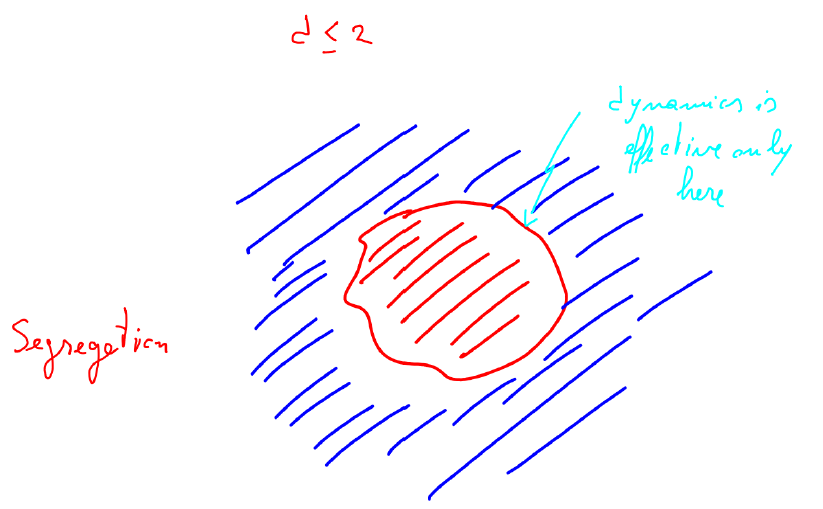
\includegraphics[width=0.8\textwidth]{\main/Images/segregation.png}
    \caption{In $d \leq 2$, different species are \textit{segregated} in regions with a high volume, and all interaction happens at their boundaries. Each of them has a high probability of getting extinct, and biodiversity is at risk. Note that, in reality, in $d=2$ we observe high biodiversity - the contrary of what the voter model would predict.}
    \label{fig:segregation}
\end{figure}

\begin{figure}[H]
    \centering
    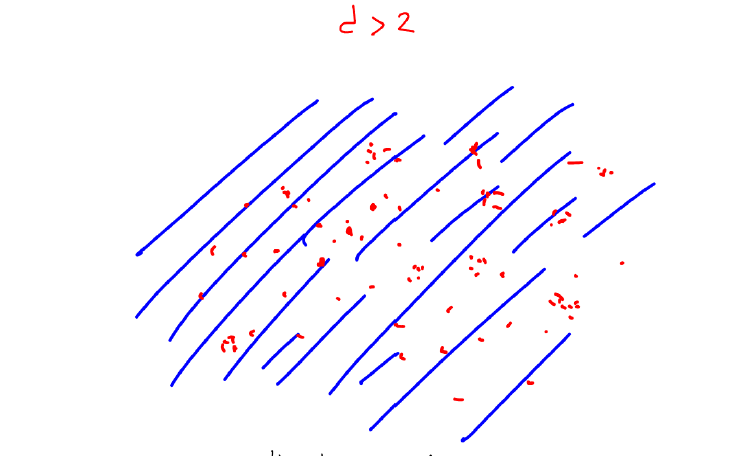
\includegraphics[width=0.8\textwidth]{\main/Images/dispersion.png}
    \caption{In $d>2$, species are \q{well mixed}, extinction events are rare and \textbf{biodiversity} is conserved.}
    \label{fig:dispersion}
\end{figure}

So, let's proceed with the necessary \textit{technical}  computations for the evolution of the $2$-point correlation function:
\begin{align}\nonumber
    \dv{t} \langle \sigma_x \sigma_y \rangle_t &= \sum_{\{\bm{\sigma}\}} \sigma_x \sigma_y \dot{\mathbb{P}}(\bm{\sigma};t) \underset{(\ref{eqn:voting-ME})}{=} \sum_z \sum_{\{\bm{\sigma}\}} \sigma_x \sigma_y [ w_z(\bm{\sigma^{(z)}}) \mathbb{P}(\bm{\sigma^{(z)}};t)- w_z(\bm{\sigma}) \mathbb{P}(\bm{\sigma};t)] =\\
    \intertext{Again we change $\bm{\sigma^{(z)}} \leftrightarrow \bm{\sigma}$ as we did in (\ref{eqn:change-trick}), so that we can write both terms in the same sum:}
    &= \sum_z \sum_{\{\bm{\sigma}\}} \mathbb{P}(\bm{\sigma};t) w_z(\bm{\sigma}) (\sigma_x^{(z)} \sigma_y^{(z)} - \sigma_x \sigma_y) \label{eqn:dt2point2}
\end{align}
Note that:
\begin{align}\label{eqn:subs}
    \begin{cases}
        \sigma_x^{(z)} \sigma_y^{(z)} = \sigma_x \sigma_y & z \neq x,y\\
        \sigma_x^{(z)} \sigma_y^{(z)} = -\sigma_x \sigma_y & z = x \> \lor \> z = y
    \end{cases} 
\end{align}
Let's consider $x \neq y$, since the $x = y$ case is trivial: $\langle \sigma_x \sigma_x \rangle \equiv 1$.

Substituting (\ref{eqn:subs}) in (\ref{eqn:dt2point2}) leads to:
\begin{align*}
    \dv{t} \langle \sigma_x \sigma_y \rangle_t &= - 2[ \langle w_x(\bm{\sigma}) \sigma_x \sigma_y \rangle_t + \langle w_y(\bm{\sigma}) \sigma_x \sigma_y \rangle_t] = \\
    &\underset{\mathclap{(\ref{eqn:spin-change2})}}{=} - \frac{\cancel{2} w}{\cancel{2} d} \Big[2d \langle \sigma_x \sigma_y  \rangle_t - \sum_{\mu=1}^d ( \langle \sigma_y \sigma_{\bm{r}_x + \bm{\hat{\mu}}} \rangle_t + \langle \sigma_y \sigma_{\bm{r}_x - \bm{\hat{\mu}}} \rangle_t) \\
    &\qquad \>\>\>\, +2d \langle \sigma_x \sigma_y \rangle_t - \sum_{\mu=1}^d (\langle \sigma_x \sigma_{\bm{r}_y + \bm{\hat{\mu}}} \rangle_t + \langle \sigma_{x} \sigma_{\bm{r}_y - \bm{\hat{\mu}}} \rangle_t) \Big]    
\end{align*}
As before, we choose $w \equiv d/4$ and rewrite the terms in the square bracket by using the discrete laplacian defined in (\ref{eqn:discrete-laplacian}), assuming translational invariance:
\begin{align*}
    4 \dv{t} G_t(\bm{r}_x - \bm{r}_y) = \bigtriangleup_{\bm{r}_x} G_t(\bm{r}_x - \bm{r}_y) + \underbrace{\bigtriangleup_{\bm{r}_y} G_t(\bm{r}_x - \bm{r}_y)}_{\bigtriangleup_{\bm{r}_x} G_t(\bm{r}_x - \bm{r}_y)} = 2 \bigtriangleup_{\bm{r}_x} G(\bm{r}_x - \bm{r}_y)
\end{align*} 

Denoting $\bm{x} \equiv \bm{r}_x - \bm{r}_y$ this becomes:
\begin{align}\label{eqn:2-point-diff-eq}
    2 \dv{t} G_t(\bm{x}) = \bigtriangleup_{\bm{x}} G_t(\bm{x}) \qquad \bm{x} \neq \bm{0}
\end{align}
with the \q{boundary condition} $G_t(\bm{0}) \equiv 1$ since $\sigma_x^2 = 1$.

\medskip

When $\bm{x}=\bm{0}$, $G_t(\bm{0})$ is constant, meaning that $\partial_t G_t(\bm{x}) = 0$. So we can rewrite (\ref{eqn:2-point-diff-eq}) to include also the $\bm{x}=\bm{0}$ case:
\begin{align*}
    2 \dv{t} G_t(\bm{x}) = (\hlc{Yellow}{1} - \hlc{SkyBlue}{\delta^d_{\bm{x},\bm{0}}}) \bigtriangleup_{\bm{x}} G_t(\bm{x})
\end{align*}
Evaluating at $\bm{x} = \bm{0}$ now leads to:
\begin{align*}
    \dv{t} G_t(\bm{x}=\bm{0}) = 0 \Rightarrow G_t(\bm{x}=\bm{0}) = \text{Constant} = G_0(\bm{x}=\bm{0}) = 1
\end{align*}

Taking the \textit{discrete} Fourier transform of both sides we get:
\begin{align}\label{eqn:2-point-diff-eq2}
    \dv{t} \tilde{G}_t(\bm{q}) = - 2\hlc{Yellow}{ \lambda(\bm{q}) \tilde{G}_t(\bm{q})} - \frac{1}{2} \hlc{SkyBlue}{\bigtriangleup_{\bm{x}} G_t(\bm{x})\Big|_{\bm{x}=\bm{0}}} 
\end{align} 
where $\lambda(\bm{q})$ is the one defined in (\ref{eqn:lambda-q}).

Unfortunately, now the $\bm{q}$ are \textit{coupled} by the blue term, and so we cannot solve directly this differential equation. To proceed, we use the \textbf{Laplace transform}, defined as follows for a generic function $f_t$:
\begin{align}\label{eqn:laplace-transform}
    \hat{f}(s) = \int_0^{+\infty} e^{-ts} f_t \dd{t} 
\end{align} 
Since the Fourier transform acts on the \textit{space} coordinates an the Laplace transform on the \textit{time} one, they commute:
\begin{align*}
    \hat{\tilde{g}}(\bm{q},s) = \tilde{\hat{g}}(\bm{q},s)
\end{align*}  

The Laplace transform of the left hand side of (\ref{eqn:2-point-diff-eq2}) gives:
\begin{align*}
    \int_0^\infty \dd{t} \dv{t} \tilde{G}_t(\bm{q}) e^{-st} &\underset{\mathclap{\text{by parts}}}{=} \tilde{G}_t(\bm{q}) e^{-s t}\Big|_{0}^\infty + s \int_0^\infty \dd{t} e^{-st} \tilde{G}_t(\bm{q}) =\\
    &\underset{\mathclap{(s > 0)}}{=} -\tilde{G}_0(\bm{q}) + s \hat{\tilde{G}}(\bm{q},s)
\end{align*}
where $\hat{\tilde{G}}(\bm{q},s)$ is the correlation function after both the Fourier and Laplace transforms:
\begin{align*}
    \hat{\tilde{G}}(\bm{q},s) \equiv \int_0^\infty \dd{t} e^{-st} \tilde{G}_t (\bm{q})
\end{align*}

And so equation (\ref{eqn:2-point-diff-eq2}) becomes:
\begin{align}\label{eqn:2-point-diff-eq3}
    s \hat{\tilde{G}}(\bm{q},s) = \tilde{G}_0(\bm{q}) - 2 \lambda(\bm{q}) \hat{\tilde{G}}(\bm{q},s) -\frac{1}{2} \bigtriangleup_{\bm{x}} \hat{G}(\bm{x},s)  \Big|_{\bm{x}=\bm{0}}
\end{align}
which is (\ref{eqn:2-point-diff-eq}) after the Fourier and Laplace transforms.

\medskip

The initial condition $\tilde{G}_0(\bm{q})$ is given by:
\begin{align}\nonumber
    \tilde{G}_0(\bm{q}) &\equiv \sum_{\bm{x}} e^{i \bm{q} \cdot \bm{x}} \langle \sigma_0 \sigma_x \rangle_{t=0} = \underbrace{1}_{x=0}  + \sum_{\bm{x} \neq \bm{0}} e^{i \bm{q} \cdot \bm{x}} \overbrace{\underbrace{\langle \sigma_0 \sigma_x \rangle}_{(2p-1)^2}}^{\text{i.i.d.} (\ref{eqn:initial-stats})}  + 1 = \\\nonumber
    &= 1 + (2p-1)^2 \sum_{\bm{x} \neq \bm{0}} e^{i \bm{q} \cdot \bm{x}}
    \intertext{Summing and subtracting $(2p-1)^2 \cdot 1$ we can extend the sum over all $\bm{x}$:} \label{eqn:in-cond-transformed}
    &= 1 - (2p-1)^2 + (2p-1)^2 \sum_{\bm{x}} e^{i \bm{q} \cdot \bm{x}} \underset{\mathclap{(\ref{eqn:e-on})}}{=}  1 - (2p-1)^2 +(2p-1)^2 L^d \delta^d_{\bm{q},\bm{0}}
\end{align}

All that's left is to compute $\bigtriangleup_{\bm{x}} \hat{G}(\bm{x},s)$ at $\bm{x}=\bm{0}$. First we rewrite the Laplace transformed $G$, i.e. $\hat{G}(\bm{x},s)$, as the Fourier anti-transform of $\hat{\tilde{G}}(\bm{q},s)$:
\begin{align*}
    \hat{G}(\bm{x},s) \underset{\mathclap{(\ref{eqn:inverse-transform})}}{=}  \frac{1}{L^d} \sum_{\bm{q}} e^{-i \bm{q} \cdot \bm{x}} \hat{\tilde{G}}(\bm{q},s) 
\end{align*}
Then we compute the laplacian:
\begin{align}\nonumber
    \bigtriangleup_{\bm{x}} \hat{G}(\bm{x},s)\Big|_{\bm{x}=\bm{0}}\> &\underset{\mathclap{(\ref{eqn:discrete-laplacian})}}{=} \sum_{\mu=1}^d [\hat{G}(\bm{\hat{\mu}}, s) + \hat{G}(-\bm{\hat{\mu}}, s) - 2 \hat{G}(\bm{0},s)] =\\ \nonumber
    &= \frac{1}{L^d} \sum_{\bm{q}} \hat{\tilde{G}}(\bm{q},s) \underbrace{\sum_{\mu=1}^d (e^{-i q_\mu} + e^{i q_\mu} - 2)}_{\sum_{\mu=1}^d 2 (\cos q_\mu -1) = -4\lambda(\bm{q})} = -\frac{4}{L^d} \sum_{\bm{q}} \lambda(\bm{q}) \hat{\tilde{G}}(\bm{q},s) =\\
    &\equiv -\frac{4}{L^d} h(s) \label{eqn:laplacian-term-transformed} \\
    h(s) &\equiv \sum_{\bm{q}} \lambda(\bm{q}) \hat{\tilde{G}}(\bm{q},s) \label{eqn:h-s}
\end{align}

Substituting (\ref{eqn:in-cond-transformed}) and (\ref{eqn:laplacian-term-transformed}) back in (\ref{eqn:2-point-diff-eq3}) and solving for $\hat{\tilde{G}}(\bm{q},s)$ we get:
\begin{align}\nonumber
    \hat{\tilde{G}}(\bm{q},s) &= \frac{\tilde{G}_0(\bm{q}) - \bigtriangleup_{\bm{x}} \hat{G}(\bm{x},s) \Big|_{\bm{x}=\bm{0}}}{s + 2 \lambda(\bm{q})} =\\
    &\underset{\mathclap{\substack{(\ref{eqn:in-cond-transformed})\\(\ref{eqn:laplacian-term-transformed})}}}{=} \frac{\tilde{G}_0(\bm{q}) + 2 L^{-d} h(s)}{s + 2\lambda(\bm{q})} 
    \label{eqn:2-point-diff-eq4}
\end{align}

However, $h(s)$ depends on $\hat{\tilde{G}}(\bm{q'},s)$ $\forall \bm{q'}$, so (\ref{eqn:2-point-diff-eq4}) is still not the solution!

\medskip

The trick is to multiply both sides by $\lambda(\bm{q})$ and sum over all $\bm{q}$. In this way, the left side becomes:
\begin{align}\label{eqn:lhs-a}
    \sum_{\bm{q}} \lambda(\bm{q}) \hat{\tilde{G}}(\bm{q},s) \underset{\mathclap{(\ref{eqn:h-s})}}{=} h(s)
\end{align}
And the right hand side:
\begin{align}\label{eqn:rhs-a}
    \sum_{\bm{q}} \frac{\lambda(\bm{q})}{s + 2 \lambda(\bm{q})}[\tilde{G}_0(\bm{q}) + 2 L^{-d} h(s)] = h(s) \underbrace{\frac{1}{L^d} \sum_{\bm{q}} \frac{2 \lambda(\bm{q})}{s + 2 \lambda(\bm{q})}}_{A(s)} + \sum_{\bm{q}} \frac{\lambda(\bm{q})}{s + 2 \lambda(\bm{q})} \tilde{G}_0(\bm{q})
\end{align}
In particular, the last term can be simplified:
\begin{align*}
    \sum_{\bm{q}} \frac{\lambda(\bm{q})}{s + 2 \lambda(\bm{q})} \tilde{G}_0(\bm{q}) &\underset{\mathclap{(\ref{eqn:in-cond-transformed})}}{=} \sum_{\bm{q}} \frac{\lambda(\bm{q})}{s + 2 \lambda(\bm{q})} \Big[1 - (2p-1)^2 +\cancel{ (2p-1)^2 \delta^d_{\bm{q},\bm{0}} L^d} \Big]
    \shortintertext{Since $\lambda(\bm{0}) = \bm{0}$:}
    &= [1-(2p-1)^2] L^d \frac{A(s)}{2} = L^d A(s) 2p(1-p) 
\end{align*}

Equating (\ref{eqn:lhs-a}) and (\ref{eqn:rhs-a}) and solving for $h(s)$ leads to:
\begin{align}\label{eqn:h-s-sol}
    h(s) = A(s)[h(s) + L^d 2p(1-p)] \Rightarrow \frac{h(s)}{L^d} = \frac{A(s)}{1-A(s)}  2p(1-p)
\end{align}
which can be substituted back in (\ref{eqn:2-point-diff-eq4}), leading to the complete solution for $\hat{\tilde{G}}(\bm{q},s)$.

%TODO Add references










\end{document}
